\documentclass[aspectratio=169, 11pt]{beamer}
\usepackage{beamer_preamble}

\begin{document}

% ==== Title ===============================================================
\titleslide{Lesson 3-5 \textperiodcentered\ Day 3 (Observation) \textperiodcentered\ Period F}{Multiplicity \& Factored-Form Graphing --- 5/8/26}

% ==== Objectives ===========================================================
\begin{frame}{Objectives}{Algebra 2 \textperiodcentered\ Lesson 3-5 \textperiodcentered\ Observation Day}
\vspace{0.15cm}
\begin{projcard}{Math Objective}{slideblue}
Construct a factored polynomial from a graph by identifying $x$-intercepts,
choosing the correct multiplicity at each (touch = even, cross = odd), and
applying end behavior to determine the leading coefficient sign.
\end{projcard}
\vspace{-0.1cm}
\begin{projcard}{Language Objective}{slidegreen}
Use the frame \textit{``The factor for $x = \underline{\hspace{0.5cm}}$ must be
$\underline{\hspace{0.5cm}}$ because the graph $\underline{\hspace{0.8cm}}$''}
to justify each factor of a polynomial.
\end{projcard}
\vspace{-0.1cm}
\begin{projcard}{Essential Understanding}{slidegold}
A polynomial's graph and its factored form encode the \textbf{same information} ---
zeros locate the factors, multiplicity determines touch vs.\ cross, and end behavior
determines the leading coefficient sign.
\end{projcard}
\end{frame}

% ==== Do Now ==============================================================
\begin{frame}{Do Now --- Quick Recall}{Algebra 2 \textperiodcentered\ Lesson 3-5 \textperiodcentered\ Observation Day}
\phasebadges{1}{5}{vocabulary recall}
\vspace{0.15cm}
\begin{projcard}{Three quick questions --- do independently:}{slidegold}
\begin{enumerate}
  \setlength{\itemsep}{0.35cm}
  \item What is the multiplicity of the zero $x = 4$ in
        $f(x) = (x-4)^2(x+1)$? \quad \underline{\hspace{2cm}}
  \item A zero with \textbf{even} multiplicity --- the graph \underline{\hspace{3cm}} the $x$-axis at that zero.
        \textit{\small (touches and turns back? crosses through?)}
  \item A zero with \textbf{odd} multiplicity --- the graph \underline{\hspace{3cm}} the $x$-axis at that zero.
\end{enumerate}
\end{projcard}
\end{frame}

% ==== Launch: phase header ================================================
\begin{frame}{Launch --- Gradual Release (15 min)}{Algebra 2 \textperiodcentered\ Lesson 3-5 \textperiodcentered\ Observation Day}
\phasebadges{1--2}{15}{I~do \textrightarrow\ you~do \textrightarrow\ I~check \textrightarrow\ we~do}
\vspace{0.2cm}
\begin{center}
{\Large\bfseries\color{slidenavy} Four steps today:}
\vspace{0.3cm}

\begin{tabular}{cl}
\tcbox[on line,colback=slidenavy,colframe=slidenavy,coltext=white,
       boxrule=0pt,arc=2pt,boxsep=2pt,left=5pt,right=5pt]{\bfseries 1} &
  \textbf{I~do} (4 min) --- teacher models with annotation \\[8pt]
\tcbox[on line,colback=slideblue,colframe=slideblue,coltext=white,
       boxrule=0pt,arc=2pt,boxsep=2pt,left=5pt,right=5pt]{\bfseries 2} &
  \textbf{You~do} (4 min) --- independent sketch \\[8pt]
\tcbox[on line,colback=slidegreen,colframe=slidegreen,coltext=white,
       boxrule=0pt,arc=2pt,boxsep=2pt,left=5pt,right=5pt]{\bfseries 3} &
  \textbf{I~check} (3 min) --- compare with exemplar \\[8pt]
\tcbox[on line,colback=slideaccent,colframe=slideaccent,coltext=white,
       boxrule=0pt,arc=2pt,boxsep=2pt,left=5pt,right=5pt]{\bfseries 4} &
  \textbf{We~do} (4 min) --- whole-class call-and-response \\
\end{tabular}
\end{center}
\end{frame}

% ==== Launch: I do =========================================================
\begin{frame}{Launch --- I~Do (4 min): Watch \& Annotate}{Algebra 2 \textperiodcentered\ Lesson 3-5 \textperiodcentered\ Observation Day}
\phasebadges{1--2}{4}{teacher models}
\vspace{0.1cm}
\begin{projcard}{Teacher example: $f(x) = (x-2)^2(x+3)$}{slidenavy}
\begin{tabular}{p{1.5in}p{3.0in}}
\textbf{Zero $x = 2$} & mult.\ = \underline{\hspace{0.6cm}}, behavior: \underline{\hspace{1.8cm}} \\[6pt]
\textbf{Zero $x = -3$} & mult.\ = \underline{\hspace{0.6cm}}, behavior: \underline{\hspace{1.8cm}} \\[6pt]
\textbf{Degree} & \underline{\hspace{0.6cm}},\quad leading coeff.\ sign: \underline{\hspace{1.3cm}} \\[6pt]
\textbf{End behavior} & left \underline{\hspace{1.2cm}}, right \underline{\hspace{1.2cm}} \\
\end{tabular}
\end{projcard}
\vspace{0.05cm}
\begin{projcard}{Touch / Cross Rule --- copy this on your packet:}{slidegreen}
\textbf{Even} multiplicity $\rightarrow$ graph \textbf{TOUCHES} $x$-axis and turns back. \\
\textbf{Odd} multiplicity $\rightarrow$ graph \textbf{CROSSES} through $x$-axis. \\
\textbf{End behavior:} degree parity + leading coeff.\ sign. Negative $\rightarrow$ down-right.
\end{projcard}
\end{frame}

% ==== Launch: You do ======================================================
\begin{frame}{Launch --- You~Do (4 min): Try This One}{Algebra 2 \textperiodcentered\ Lesson 3-5 \textperiodcentered\ Observation Day}
\phasebadges{1--2}{4}{independent work}
\vspace{0.2cm}
\begin{projcard}{Sketch $g(x) = (x+1)(x-4)^2$ on the grid in your packet.}{slideblue}
\begin{enumerate}
  \setlength{\itemsep}{0.2cm}
  \item Identify each zero and its multiplicity.
  \item Label each zero as \textbf{touch} or \textbf{cross} using the rule.
  \item Determine end behavior and sketch the curve.
\end{enumerate}
\vspace{0.2cm}
\small\textcolor{slidegray}{No computing exact $y$-values --- sketch the shape only.
Use the rule you just copied.}
\end{projcard}
\end{frame}

% ==== Launch: I check =====================================================
\begin{frame}{Launch --- I~Check (3 min): Compare \& Revise}{Algebra 2 \textperiodcentered\ Lesson 3-5 \textperiodcentered\ Observation Day}
\phasebadges{1--2}{3}{compare with exemplar}
\vspace{0.2cm}
\begin{projcard}{Exemplar for $g(x) = (x+1)(x-4)^2$}{slidegreen}
\begin{tabular}{p{1.6in}p{3.0in}}
\textbf{Zero $x = -1$} & multiplicity 1 $\rightarrow$ \textbf{CROSS} \\[5pt]
\textbf{Zero $x = 4$} & multiplicity 2 $\rightarrow$ \textbf{TOUCH} \\[5pt]
\textbf{Degree 3, pos.\ coeff.} & ends: left \textbf{down}, right \textbf{up} \\
\end{tabular}
\end{projcard}
\vspace{0.15cm}
\begin{projcard}{What did you fix? Write it in your packet.}{slidegold}
\textit{Common error:} crossing at $x = 4$ instead of touching. \\[4pt]
\textit{Why it matters:} the squared factor $(x-4)^2$ always bends back --- it cannot cross.
\end{projcard}
\end{frame}

% ==== Launch: We do =======================================================
\begin{frame}{Launch --- We~Do (4 min): Call \& Response}{Algebra 2 \textperiodcentered\ Lesson 3-5 \textperiodcentered\ Observation Day}
\phasebadges{1--2}{4}{whole-class}
\vspace{0.2cm}
\begin{projcard}{Class example: $h(x) = -x(x+2)^2(x-1)$ --- fill in as we go:}{slideaccent}
\begin{tabular}{p{1.5in}p{3.0in}}
\textbf{Zeros} & $x = $ \underline{\hspace{0.5cm}}, \underline{\hspace{0.5cm}}, \underline{\hspace{0.5cm}} \\[6pt]
\textbf{Touch or cross?} & $x=0$: \underline{\hspace{1.2cm}}\quad $x=-2$: \underline{\hspace{1.2cm}}\quad $x=1$: \underline{\hspace{1.2cm}} \\[6pt]
\textbf{Degree \& sign} & degree = \underline{\hspace{0.5cm}},\quad leading coeff.\ = \underline{\hspace{0.5cm}} \\[6pt]
\textbf{End behavior} & left \underline{\hspace{1.2cm}}, right \underline{\hspace{1.2cm}} \\
\end{tabular}
\vspace{0.1cm}
\small\textcolor{white}{Negative leading coefficient, degree 4: both ends DOWN.}
\end{projcard}
\end{frame}

% ==== Touch/Cross Rule (highlighted) =====================================
\begin{frame}{The Touch / Cross Rule}{Algebra 2 \textperiodcentered\ Lesson 3-5 \textperiodcentered\ Observation Day}
\vspace{0.25cm}
\begin{projcard}{TOUCH / CROSS RULE --- the key to today's task:}{slidegreen}
\begin{tabular}{cl}
\tcbox[on line,colback=slideblue,colframe=slideblue,coltext=white,
       boxrule=0pt,arc=3pt,boxsep=3pt,left=6pt,right=6pt]{\bfseries EVEN} &
  \textbf{TOUCHES} the $x$-axis and turns back \textit{(squared, quartic, $\ldots$)} \\[10pt]
\tcbox[on line,colback=slideaccent,colframe=slideaccent,coltext=white,
       boxrule=0pt,arc=3pt,boxsep=3pt,left=6pt,right=6pt]{\bfseries ODD} &
  \textbf{CROSSES} through the $x$-axis \textit{(linear, cubic, $\ldots$)} \\[14pt]
\tcbox[on line,colback=slidegold,colframe=slidegold,coltext=white,
       boxrule=0pt,arc=3pt,boxsep=3pt,left=6pt,right=6pt]{\bfseries SIGN} &
  Leading coeff.\ $+$ $\rightarrow$ ends \textbf{up-right};
  leading coeff.\ $-$ $\rightarrow$ ends \textbf{down-right} \\
\end{tabular}
\end{projcard}

\vspace{0.2cm}
\begin{projcard}{Quick self-check before Explore:}{slidenavy}
Read a factor, name its multiplicity, call touch or cross --- in 3 seconds.\\
If you cannot, revisit the rule card in your packet \textit{now}.
\end{projcard}
\end{frame}

% ==== Explore: Mystery Graph (task) ========================================
\begin{frame}{Explore --- Mystery Graph DOK-3 (10 min TPS)}{Algebra 2 \textperiodcentered\ Lesson 3-5 \textperiodcentered\ Observation Day}
\phasebadges{3}{10}{think-pair-share}
\vspace{0.1cm}
\begin{columns}[T]
\column{0.52\textwidth}
\begin{projcard}{The Graph}{slideaccent}
\begin{center}
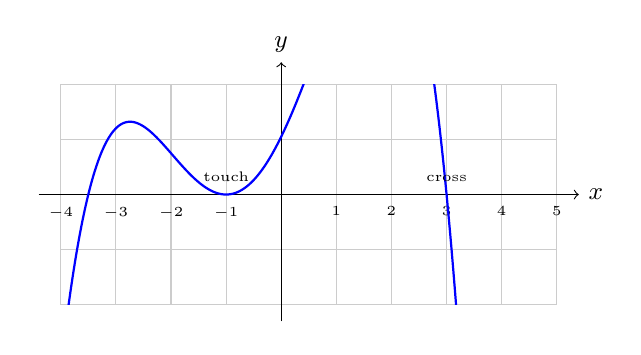
\begin{tikzpicture}[scale=0.70]
  \draw[thin,gray!40] (-4,-2) grid (5,2);
  \draw[->] (-4.4,0) -- (5.4,0) node[right] {\small $x$};
  \draw[->] (0,-2.3) -- (0,2.4) node[above] {\small $y$};
  \foreach \x in {-4,-3,-2,-1,1,2,3,4,5}
    \node[below,font=\tiny] at (\x,-0.05) {$\x$};
  \begin{scope}
    \clip (-4,-2) rectangle (5,2);
    \draw[thick,blue,domain=-4:5,samples=300,smooth]
      plot (\x, {-0.10*(\x+1)*(\x+1)*(\x-3)*(\x+3.5)});
  \end{scope}
  \node[font=\tiny,above] at (-1,0.05) {touch};
  \node[font=\tiny,above] at (3,0.05) {cross};
  \path[use as bounding box] (-4.6,-2.4) rectangle (5.6,2.6);
\end{tikzpicture}
\end{center}
\small Zeros at $x=-1$ \textbf{(touch)} and $x=3$ \textbf{(cross)}.\\
\textbf{Both ends point downward.}
\end{projcard}

\column{0.46\textwidth}
\begin{projcard}{Your task:}{slidenavy}
\textbf{Build a possible factored form.}\\
\textbf{Justify every piece.}

\vspace{0.25cm}
\begin{enumerate}
  \setlength{\itemsep}{0.15cm}
  \item Factor for $x=-1$: why?
  \item Factor for $x=3$: why?
  \item Leading coefficient sign: why?
  \item Could the degree differ?
\end{enumerate}

\vspace{0.2cm}
\small\textcolor{slidegray}{3 min alone $\rightarrow$ 3 min partner
$\rightarrow$ 4 min whole-class.}
\end{projcard}

\end{columns}
\end{frame}

% ==== Explore: Mystery Graph reasoning prompts ============================
\begin{frame}{Explore --- Mystery Graph: Whole-Group Synthesis}{Algebra 2 \textperiodcentered\ Lesson 3-5 \textperiodcentered\ Observation Day}
\phasebadges{3}{4}{whole-group debrief}
\vspace{0.15cm}
\begin{projcard}{Press on these in the debrief:}{slideaccent}
\begin{enumerate}
  \setlength{\itemsep}{0.3cm}
  \item Where does the graph \textbf{touch} vs.\ \textbf{cross}? What does each tell you about the exponent of that factor?
  \item What does \textbf{both ends down} tell you about the degree and leading coefficient sign?
  \item Why must the leading coefficient be \textbf{negative}?
  \item Could the degree be 4 instead of 3? What would change?
  \item How would you check your factored form using Desmos?
\end{enumerate}
\end{projcard}
\vspace{0.1cm}
\small\textcolor{slidegray}{Use sentence frames: ``The factor for $x = \underline{\hspace{0.4cm}}$ must be $\underline{\hspace{0.6cm}}$ because the graph $\underline{\hspace{0.6cm}}$.'' Cold-call a pair who used the frame.}
\end{frame}

% ==== Explore: DOK-2 consolidation ========================================
\begin{frame}{Explore --- DOK-2 Consolidation (15 min, partners)}{Algebra 2 \textperiodcentered\ Lesson 3-5 \textperiodcentered\ Observation Day}
\phasebadges{2}{15}{partner work}
\vspace{0.15cm}
\begin{projcard}{Three items in order --- work with your partner:}{slideblue}
\begin{enumerate}
  \setlength{\itemsep}{0.4cm}
  \item \textbf{(Savvas q12)} Sketch $f(x) = 3x^3 - 9x^2 - 12x$.
        Find zeros first (factor it), then label touch / cross.
  \item \textbf{(Try-It 2b)} Describe behavior at each zero of
        $f(x) = (x^2+9)(x-1)^5(x+2)^2$.
        \textit{What is $(x^2+9)$?}
  \item A graph crosses at $x = 0$, touches at $x = 2$, both ends up.
        Write a possible factored form. Justify the leading coeff.\ sign.
\end{enumerate}
\vspace{0.15cm}
\small\textcolor{slidegray}{Record reasoning, not just answers.
Verify with Desmos at the end of each item.}
\end{projcard}
\end{frame}

% ==== Sentence Frames =====================================================
\begin{frame}{Sentence Frames (ELL Support --- use these when you share)}{Algebra 2 \textperiodcentered\ Lesson 3-5 \textperiodcentered\ Observation Day}
\vspace{0.3cm}
\begin{projcard}{Use these frames throughout today's tasks:}{slidegreen}
\vspace{0.2cm}
\begin{enumerate}
  \setlength{\itemsep}{0.5cm}
  \item ``The factor for $x = \underline{\hspace{0.7cm}}$ must be $\underline{\hspace{0.7cm}}$
        because the graph $\underline{\hspace{1.4cm}}$.''
  \item ``The leading coefficient is $\underline{\hspace{0.7cm}}$ because the ends
        go $\underline{\hspace{1.2cm}}$.''
  \item ``I notice $\underline{\hspace{1.4cm}}$, so I think $\underline{\hspace{1.4cm}}$.''
\end{enumerate}
\end{projcard}
\end{frame}

% ==== Share / Summary =====================================================
\begin{frame}{Share / Summary (5 min)}{Algebra 2 \textperiodcentered\ Lesson 3-5 \textperiodcentered\ Observation Day}
\phasebadges{1--2}{5}{synthesis}
\vspace{0.15cm}
\begin{projcard}{Today's rule, one more time:}{slidegreen}
\textbf{Even} multiplicity $\rightarrow$ TOUCH \quad\textbf{Odd} multiplicity $\rightarrow$ CROSS\\
\textbf{Leading coeff.\ sign} + \textbf{degree parity} $\rightarrow$ END BEHAVIOR
\end{projcard}
\vspace{0.1cm}
\begin{projcard}{Objectives --- which did you hit today?}{slideblue}
\begin{itemize}
  \setlength{\itemsep}{0.1cm}
  \item[$\square$] \textbf{Math:} Construct a factored polynomial from a graph (zeros + multiplicity + end behavior).
  \item[$\square$] \textbf{Language:} Used the sentence frame to justify each factor.
  \item[$\square$] \textbf{Essential Understanding:} Graph and factored form encode the same information.
\end{itemize}
\end{projcard}
\vspace{0.1cm}
\begin{projcard}{Next class (Mon 5/11):}{slidegold}
Storage Box DOK-3 --- real + complex zeros and volume modeling.
\end{projcard}
\end{frame}

% ==== Exit Ticket =========================================================
\begin{frame}{Exit Ticket --- DOK-1 Cool-Down (5 min)}{Algebra 2 \textperiodcentered\ Lesson 3-5 \textperiodcentered\ Observation Day}
\phasebadges{1}{5}{not graded --- turn in at door}
\vspace{0.2cm}
\begin{projcard}{Complete independently on the exit ticket strip:}{slidegold}
\begin{enumerate}
  \setlength{\itemsep}{0.35cm}
  \item A factor of $(x-4)^2$ produces a \underline{\hspace{2cm}} at $x = 4$.
        \hfill\textit{\small (touch / cross)}
  \item A factor of $(x+1)$ produces a \underline{\hspace{2cm}} at $x = -1$.
        \hfill\textit{\small (touch / cross)}
  \item \textbf{The biggest thing I learned today was:}
        \underline{\hspace{4.5cm}}
\end{enumerate}
\end{projcard}
\end{frame}

% ==== Closing =============================================================
\begin{frame}[plain]
{\setbeamercolor{background canvas}{bg=slidenavy}
\color{white}
\vspace{2cm}
\begin{center}
{\fontsize{26pt}{30pt}\selectfont\bfseries Lesson 3-5 \textperiodcentered\ Day 3}\\[0.6cm]
{\Large Multiplicity \& Factored-Form Graphing}\\[0.8cm]
{\normalsize\color{slidelight} Period F \textperiodcentered\ May 8, 2026}\\[0.4cm]
{\normalsize\color{slidelight!70}
  Observation context: gradual-release Launch fidelity + DOK-3 Mystery Graph spine.\\
  Thank you for visiting.}
\end{center}
}
\end{frame}

\end{document}
